
To assess the risk of disclosure, we use a measure proposed by \citep{KinneyEtAl2011}: For each industry, we estimate the fraction of entities by industry for which the synthetic birth year equals the true birth year, conditional on the synthetic birth year, and interpret it as a probability. Tables~\ref{tab:Can:ProbabilityPrivate} and \ref{tab:GLBD:Probability} in the appendix show the minimum, maximum, and mean of these probabilities, by year. Figure~\ref{fig:Conf.Both} shows the maximum and average values across time, for each country.\footnote{The Canadian manufacturing sector is not shown. In the German case, we only use two industries, but we show the average of the two, rather than the values for both industries, to maintain comparability with the Canadian plot.} The figure shows that these probabilities are quite low except for the first year. As Figure~\ref{fig:FirmDynamics} showed, entry rates in the first year are much larger than in any other year due to censoring. It is therefore quite likely that the (left-censored) entry year of the synthetic record matches that of the (left-censored) original record if the synthetic entry year is the first year observed in the data. A somewhat more muted version of this effect can be seen for Germany in the years 1991 and 1992, when the lower panel of %Table~\ref{tab:GLBD:Probability} 
Figure~\ref{fig:Conf.Both} shows another spike. These are the years in which data from Eastern Germany were added to the database successively, leading to new sets of (left-censored) entities. 

With the exception of the first year in the data, the average rate of concordance between synthetic and observed birth year of an establishment in the Canadian data is below 5\%, and the maximum is never above 50\%. The German data reflect results from a smaller set of industries, and while the average concordance is higher (never above 10\%), the maximum is never above 6\% other than during the noted entry spikes. This suggests that the synthetic lifespan of any given entity is highly unlikely to be matched to its confidential real lifespan. This is generally considered to be a high degree of confidentiality. 


\begin{figure}[ht]
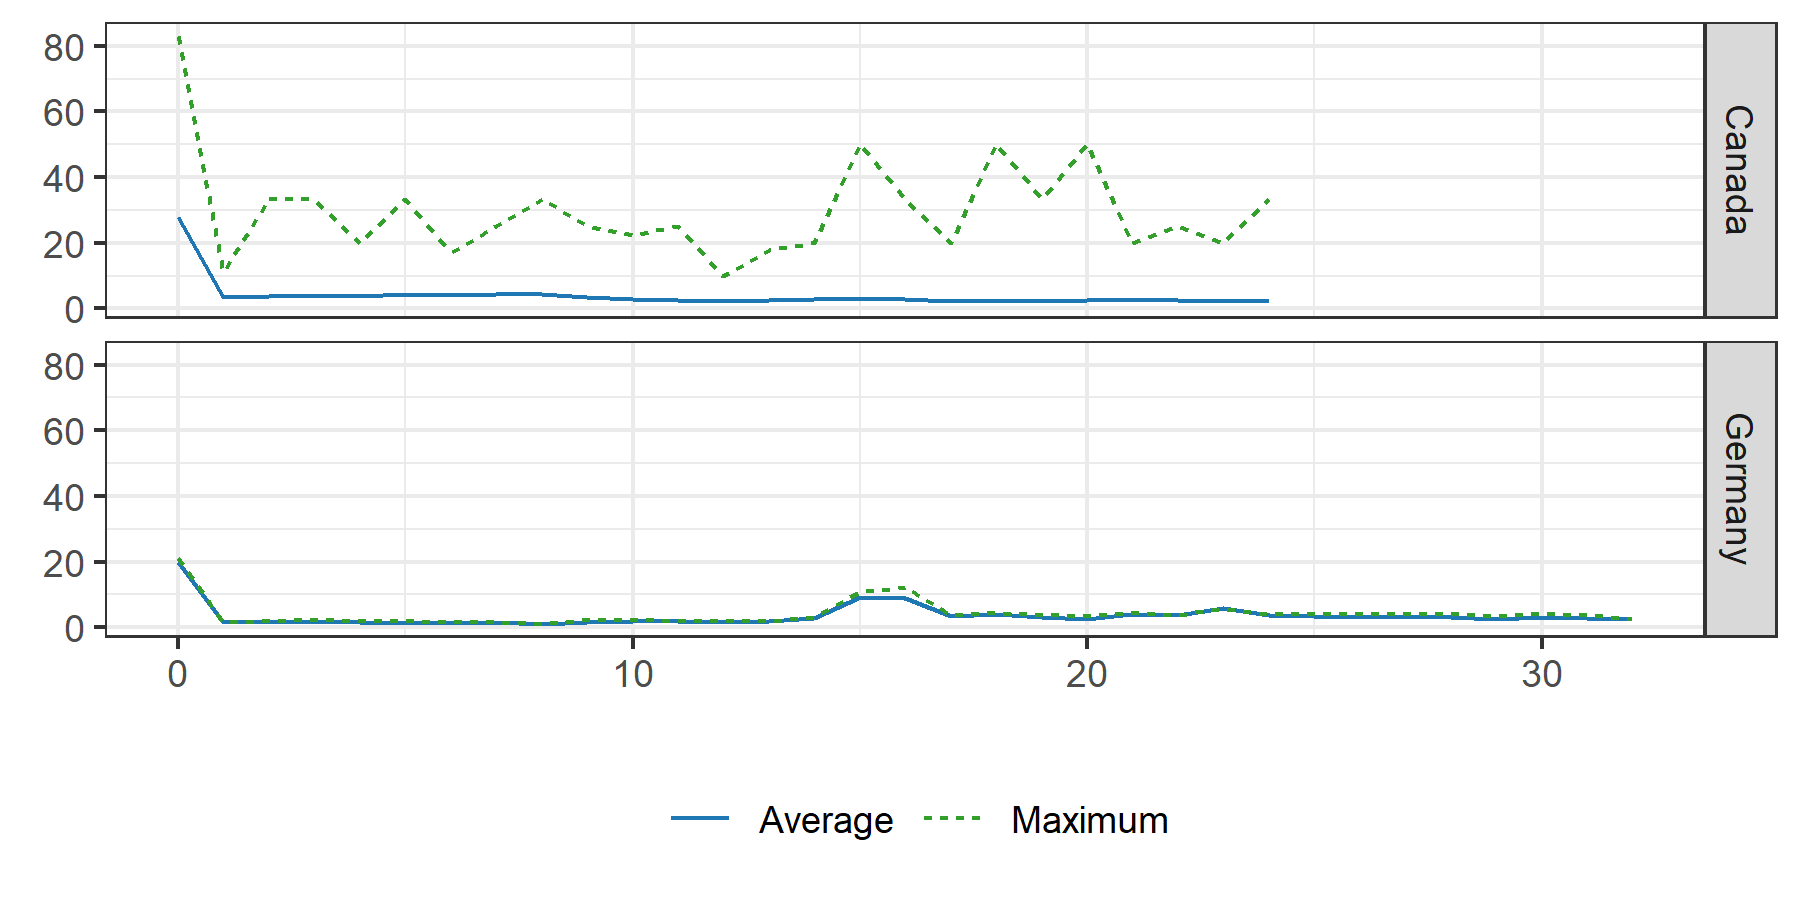
\includegraphics[width=\linewidth]{r-graphs/fig_conf_both.png}
\caption{Average and maximum likelihood that synthetic birthyear matches actual birthyear\label{fig:Conf.Both}}

\begin{center}
\begin{minipage}{0.8\linewidth}
	\footnotesize \it
Plot shows fraction of entities by industry for which the synthetic birth year equals the true birth year, conditional on the synthetic birth year, and interpret it as a probability. Plot has been rescaled to be relative to the first year observed in the data.	
\end{minipage}
\end{center}
\end{figure}


% WANT: Graphs

% Question: in Germany, with only two industries, how do we get three values?
